
Linux là một hệ điều hành mã nguồn mở (open-source OS) chạy trên hầu hết các kiến trúc vi xử lý, bao gồm dòng vi xử lý ARM. Linux được hỗ trợ bởi một cộng đồng mã nguồn mở (GNU), chính điều này làm cho Linux rất linh hoạt và phát triển rất nhanh với nhiều tính năng không thua kém các hệ điều hành khác hiện nay. Tất cả các ứng dụng chạy trên hệ điều hành UNIX đều tương thích với Linux.

Hầu hết các bản Linux đều hỗ trợ rất nhiều ngôn ngữ lập trình, đặc biệt công cụ GCC cho phép người lập trình có thể biên dịch và thực thi ứng dụng viết bằng nhiều ngôn ngữ lập trình khác nhau: C/C++, Java, .v.v... Ngoài ra, Linux còn hỗ trợ ngôn ngữ lập trình để phát triển các ứng dụng đồ họa như: JTK+, Qt, .v.v...

Do chi phí thấp, khả năng thay đổi tương thích với phần cứng dễ dàng nên nhúng Linux thường được sử dụng rất nhiều trong các hệ thống nhúng (embedded system). Ngày nay, Linux đã trở thành một đối thủ cạnh tranh lớn về lĩnh vực hệ điều hành trong các dòng điện thoại thông minh (smartphone), các thiết bị PDA (personal digital assistant) và là một lựa chọn thay thế cho sự độc quyền của Windows CE và Palm OS.

Theo định nghĩa của IEEE (Hiệp hội kỹ sư điện và điện tử Hoa kỳ): Hệ thống nhúng là một phần của hệ thống lớn hơn và thực hiện một số chức năng của hệ thống đó.

Đặc trưng của hệ điều hành nhúng:
\begin{itemize}
	\item Tăng tính tin cậy (reliability)
	\item Tăng tính khả chuyển (portability)
	\item Khả năng tương thích mềm: dễ dàng nâng cấp hay thu gọn để tương thích với nền tảng hệ thống
	\item Cung cấp các cơ chế lập lịch (scheduler) hỗ trợ thời gian thực (Realtime OS – RTOS)
\end{itemize}
\begin{figure}[H]
	\centering
	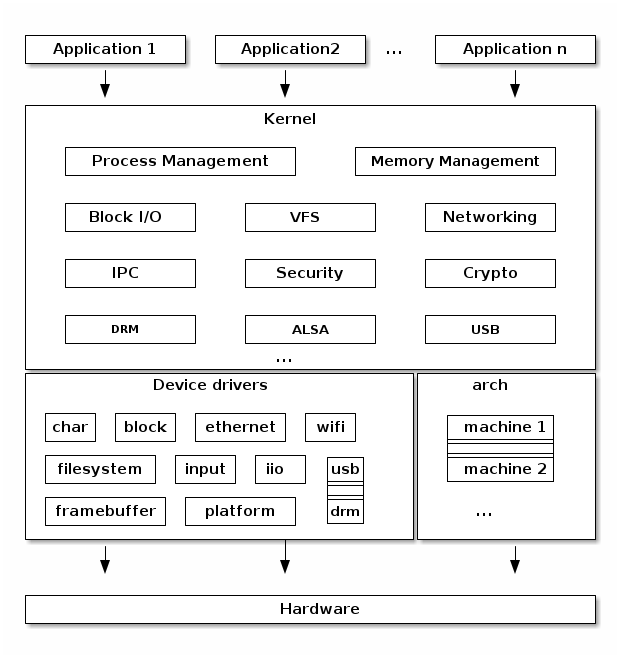
\includegraphics[width=0.8\textwidth]{../images/cau-truc-linux.png}
	\caption{Cấu trúc hệ điều hành}
\end{figure}
